\documentclass[11pt]{article}
\usepackage[top=1.00in, bottom=1.0in, left=1.1in, right=1.1in]{geometry}
\renewcommand{\baselinestretch}{1.1}
\usepackage{graphicx}
\usepackage{natbib}
\usepackage{amsmath}
\usepackage{gensymb}
\usepackage[utf8]{inputenc}
\usepackage{parskip}
\usepackage{hyperref}
\usepackage{longtable}

\def\labelitemi{--}
\parindent=0pt

\begin{document}

\renewcommand{\refname}{\CHead{}}

\begin{center}
{\sc Supplementary Information for:} {\Large Why longer seasons with climate change \\ may not always increase tree growth} \\
\vspace{5ex}
{\sc Authors:} E.M. Wolkovich$^1$, Ailene K. Ettinger$^2$, Alana Chin$^3$, Catherine J. Chamberlain$^4$,\\ Frederik Baumgarten$^1$, Kavya Pradhan$^{5,6}$, Rub{\'e}n D. Manzanedo$^{7-9}$ \&  Janneke Hille Ris Lambers$^7$
\end{center}

\renewcommand{\thetable}{S\arabic{table}}
\renewcommand{\thefigure}{S\arabic{figure}}


\section*{Literature review methods}

We conducted a review to find papers focused on relationships between growing season length and tree wood growth, though contrasting terminology made it challenging to identify papers through one search. After reviewing several recent papers \citep{dow2022warm,zohner2023effect}, we searched ISI Web of Science for ``growing season length" AND ``tree ring*" (ALL FIELDS) on 12 April 2023, which returned 33 citations. We next reviewed abstracts from these papers and discarded ones that did not mention the relationship between growing season length and growth. We further reviewed all citations within all papers for additionally relevant papers and included them in our review following the same criteria of reviewing abstracts and including papers that mentioned they tested or examined the relationship between growing season length and tree growth. Papers needed at least one metric related to growing season length and one metric related to growth to be included (and these could not be the same metric) but we did not require they clearly measure season length (end and start) to be included. In total we report on 36 papers after reviewing over 107 potentially relevant papers and discarding one paper from which we scraped data but found it did not meet our criteria \citep[][because it used tree rings as a metric of both growth and growing season length]{bruening2017}. 

Once a paper was included, we aimed to record all studies from it related to season length and growth (e.g. a paper might include a global study of satellite metrics of start of season and productivity as well as an experiment; these would be considered two separate studies within one paper). Given the large diversity of metrics we found, we did not extract quantitative estimates of growing season length, growth, or their relationship. Instead, we extracted data on location, species, how they measured growing season length, growth, what relationship they found and what internal and external drivers they mentioned (full dataset with metadata details for each column available on the Knowledge Network for Biocomplexity at publication). 

Papers often reported dozens or more statistical tests from different analyses of data or different types or subsets of data, thus we recorded a unique observation (that is, one recorded row of data for our literature review) within each study when papers reported: (1) distinctly different datasets (e.g., a global analyses of observations and a short-term experiment); (2) multiple distinctly different measures of growth (e.g., tree ring width and flux tower) and/or growing season length (e.g., they reported both end of season as budset and end of wood growth through xylogenesis); (3) distinctly different results for growth $\times$  growing season length depending on metric (e.g., using budset for growing season length they find a growth $\times$ growing season length relationship, but using leaf coloring they do not). 

We returned to the papers to also assess them for which hypotheses they addressed. For this, we reviewed papers for stated hypotheses and/or analogous research questions that were specifically addressed in the results (e.g. hypothesis testing).  After this we grouped each hypothesis to a broader main hypothesis (or hypothesis cluster) displayed in Fig. 1, save for hypotheses including $CO_2$ limitation, which is not shown but mentioned in three papers (see Table \ref{tab:ref}). We extracted all hypotheses/questions from each paper, resulting in many papers addressing multiple hypotheses (11 of 36 papers). 

\subsection*{Trends with year}
Across studies that found support for or against a relationship between growth and growing season length (40 of 59 total studies) the range of years was very similar: spanning 2000 to 2023 with a mean of 2017 for studies that found a positive relationship and spanning 2012 to 2023 with a mean of 2020 for studies that did not. Further, we found no trend through time for finding a positive or negative relationship  (estimated slope from logistic regression overlapped 0). 

\section*{Growth $\times$ elevation relationships}

Using Google Scholar and ISI Web of Science, we searched the literature for studies of tree growth, especially via diameter or ring width, by elevation or latitude. Of 20 papers we found for these relationships, six included clear raw tree data in either scatterplots or tables that we scraped: \cite{oleksyn1998growth,huang2010radial,cavin2017highest,wang2017climatic,zhu2018spatial,zhou2022altitudinal}. 

We could not scrape data from 14 papers for the following reasons: 
\begin{enumerate}
\item Absence of observational tree growth raw data: Some studies only presented the correlation or the data was modeled. 
\item  Measures other variables: Some studies examined leaf area index and forest NPP. 
\item  Standardization of tree growth with other variables: Papers did not present the raw data (e.g., papers presented the data calculated with other variables).
\item  Presence of overlapping data points: Data points in the plots presented were not visually identifiable for accurate data scraping.
\item Line graphs: No discrete data points for image processing. 
\item Geographical scale: The locations of data collection spread across large longitudinal or latitudinal gradient. 
\end{enumerate}

We scraped tree growth data from the selected studies using the Fiji image processing package with the Figure Calibration plugin. We calibrated $x$ and $y$ axes using the Figure Calibration plugin, followed by measuring growth values at different elevation using the measure function in Fiji. Of the six remaining papers, we show results for three, excluding \cite{huang2010radial} because it included only results for trends by latitude (and most other studies included only trends by elevation), and \cite{cavin2017highest,zhu2018spatial} because the elevation co-varied with latitude. 

Thus, we show data from: \cite{oleksyn1998growth}, which measured 54 populations of  \emph{Picea abies} along 8 altitudinal transects in Southern Poland, we present the mean DBH (cm yr$^{-1}$) of values collected from each population (although 54 populations were monitored, only 42 data points were clearly visible in Figure 2 in the paper); \cite{wang2017climatic}, which collected  tree cores (37-100 years) collected from 4 different sites across an elevation gradient in the Luyashan Mountains in North China, we present the median of tree ring width values from the collected cores (147 tree cores collected from 73 trees); and \cite{zhou2022altitudinal}, who collected tree ring width data (cores of 60-80 years) of \emph{Pinus yunnar} from 6 altitudinal transects in Yunnan, China; we present the median of tree ring width of each transect.

\section*{The challenge of metrics: Measuring growth and growing season length}

Understanding the diverse drivers and testing underlying hypotheses (Fig. 1) for growth $\times$ season length relationships requires a common language. We found 14 different metrics of start of season, 16 metrics of end of season (25 metrics of growing season length), and 21 different metrics of growth across 59 studies---highlighting just part of the problem (see also \emph{Box: Growth, season length and the challenge of standardized metrics} in the main text). Definitions and metrics for external and internal drivers were myriad, 
with papers reporting dozens of tests of different aspects of climate over different temporal windows. Although this is understandable given the differing goals of these papers, it also slows progress. 

A common framework for explanatory and response variables would accelerate research by easing communication between fields and providing a path to comparable quantitative estimates. 
This should also include expected statistical tests, as we found a number of papers failed to directly test for growth $\times$ growing season length relationships (Fig. 2), often instead testing only certain hypothesized indirect relationships \citep[e.g. spring temperature $\times$ growth in][]{dow2022warm}. 

\subsection*{Measuring growth}

Tree growth can be defined and measured in a variety of ways. It is often divided into primary (growth from the root and shoot tips that results in increased height and length) versus secondary (growth that increases the thickness or girth of stems and branches above ground, as well as below ground parts), or leaf production versus wood production. Across studies, we found the largest proportion used metrics related to secondary growth ($n=$28), followed by primary growth ($n=$20), with a smaller number used metrics that reflect combined primary and secondary growth, including biomass, height, or number of stems ($n=$9), and root:shoot ratio ($n =$1).  Other studies used modeled estimates of photosynthesis (e.g., \cite{smith2014implications} relied on daily photosynthesis estimates derived from the LPJ-GUESS photosynthesis model, while \cite{chen2000approaches} estimated photosynthesis using the Integrated Terrestrial Ecosystem C-budget model, InTEC). 
Others measured photosynthesis at the leaf level, through flux towers, or used greenness metrics (NDVI). 

Growth measurements varied across disciplines and study types, posing further challenges to an interdisciplinary approach to understanding how growing season length relates to growth. 
Greenhouse or growth chamber studies and provenance trials were more likely to measure height or biomass, whereas larger scale syntheses and remote-sensed studies are more likely to use metrics of carbon assimilation. 
The inconsistency of current metrics across fields is not surprising, but may be confusing---including photosynthesis as a metric of growth may seem unconventional for ecophysiologists, for example, who may interpret the process of photosynthesis as distinct from growth---and also stalls progress toward a unified model across disciplines.

Aligning across the range and scale of growth metrics will be critical for an integrated understanding of growth-growing season length relationships and implications under continued climate change.  
There is decoupling among some metrics of growth, as different types of growth (leaves, shoots, wood) have different phenologies within a season, and may vary across years, as well (e.g., with different lags, ED Fig. 1).
For example, vegetation photosynthesis may be poorly correlated with tree radial growth, and this relationship can vary seasonally \citep{cabon2022cross}. 
Further, tree radial growth is not a perfect indicator of whole tree growth, since plants allocate carbon to their roots, leaves, reproductive structures, and stores in addition to aboveground biomass. 
Relationships among different metrics of growth are not simple, so selecting relevant ones and aligning across the most widely used ones will be necessary, though not easy: the relationship  between photosynthesis, radial growth, and carbon uptake has large implications for future carbon sequestration and it remains widely debated \citep{green2022limits}. 
Further, there is a need to understand how to scale up across these varying metrics- from leaf and individual level to populations, communities, and ecosystems- while incorporating the variation that exists within and across levels.

\subsection*{Measuring growing season length}

Growing season length is defined in myriad ways due to varying definitions and metrics for the start of season and the end of season. For example, the end of season could be defined as budset, representing the end of vegetative phenology, or as xylogenesis, representing the end of wood phenology. Additionally, in our literature review, we found several studies that leveraged climate data as a proxy for start or end of season metrics, such as snowmelt for start of season or growing season GDDs. We therefore grouped all reported growing season length metrics into four separate categories: 1) `Climate and date' simulated by climate data, 2) `Vegetative phenology' through field observations or satellite derived measurements, 3) `Wood phenology' measured by dendrometers and xylogenesis, and 4) not measured, which includes all studies that only measured start or end of seasons but not both. We found a diversity of metrics of GSL (see `Box. Defining growth, growing season length and the quest for a comprehensive framework across external and internal drivers' in main text) which were generally simplified and could not be easily aligned, as we found 14 different metrics of start of season and 16 metrics of end of season, resulting in  25 metrics of growing season length. 

\section*{Extending disciplinary focus to help bridge the internal-external drivers divide} 

Each field studying growth $\times$ growing season length today has its own historical aims, and thus, its own biases towards certain species, methods and metrics. For example, dendrochronology's original focus on using tree growth to estimate climate has led to sampling biases \citep[e.g. to `climate-sensitive' individual trees,][]{klesse2018sampling,nehrbass2014influence} and statistical detrending \citep{rollinson2021climate}, which may obscure patterns where the signal of longer growing seasons and biotic drivers may be most apparent (such as rapid growth phases). Dendrochronology also generally focuses on conifers \citep[gymnosperms,][]{zhao2019international}, creating a major split from most studies of leaf phenology, which focus almost entirely on deciduous angiosperm species (see ED Fig. 4). By contrast, phenology research has been strongly focused on spring events (e.g. budburst, leafout), with limited data on fall events and thus limited data to calculate growing season length. This focus on spring events may have been justified decades ago, when most shifts from anthropogenic warming occurred in the spring, but less justified as increasing research suggests important complexity in fall shifts \citep{gill2015,zohner2023effect} and a need to scale up phenological research to understand tree growth.

These field-specific historical trends limit the opportunities for interdisciplinary insights. For example, dendrochronology studies generally eliminate much of the drivers that physiological studies focus on, while physiological studies often fail to make predictions that scale up (e.g., to adult trees or for diverse species). Opportunities to overlap dendrochronology time records with metrics of growing season length measured through vegetative phenology appear high (ED Fig. 4), but sampling biases towards conifers in one and angiosperms in the other field limit current opportunities. All fields could therefore benefit from tackling the challenge of understanding the physiological connections between growing season length and growth, and even the genetic and developmental underpinnings of these connections. To date, much work has focused on measures of growth and phenology without a clear mechanistic understanding of what triggers growth and its cessation, and how these triggers and responses have evolved.  
Progress in this area could be particularly important for making projections, as extrapolating can be dangerous when the underlying mechanistic model is wrong. Physiological studies that follow carbohydrate balance and cell division \citep[see][]{locosselli2017dendrobiochemistry} versus growth dynamics could yield insights, as could additional work on xylogenesis---especially if done with a focus both to extrapolate to long-term tree ring studies and/or in physiological experiments \citep{fang2020physiological,simard2013intra}. Expanding beyond the current disciplines focused on this topic could also be informative. For example, a clearer physiological understanding of which environmental stimuli trigger leaf expansion, senescence, woody growth, and heartwood formation alongside an evolutionary perspective could advance understanding of growth
constraints \citep{baas2011wood,eckert2019makes,ensminger2015tree,juvany2013photo}.


\clearpage
\section*{Figures \& Tables}

% latex table generated in R 4.4.3 by xtable 1.8-4 package
% Wed Aug 27 15:40:17 2025
\begingroup\footnotesize
\begin{longtable}{p{0.3\textwidth}p{0.1\textwidth}p{0.40\textwidth}}
\caption{\textbf{Hypotheses and references for studies in our database.}} \\ 
  \hline
Hypothesis & Number of Studies & References \\ 
  \hline \endhead  \hline
longer season = more growth &  10 & \citep{camarero2022decoupled,chen2000,vcufar2015variations,delpierre2017tree,de2022temperature,gao2022earlier,grossiord2022warming,keenan2014net,silvestro2023longer,wheeler2016snow} \\ 
  warmer temperatures = more drought (drought limitation) &  10 & \citep{brand2022,buermann2018widespread,camarero2022decoupled,de2022temperature,drew2018growth,eckes2021,etzold2022number,kolavr2016response,oddi2022contrasting,zhu2021different} \\ 
  warmer temperatures = more growth &   8 & \citep{camarero2022decoupled,dow2022warm,finzi2020,moser2010timing,richardson2010influence,soolanayakanahally2013timing,stridbeck2022,zhang2021drought} \\ 
  shift of whole pheno sequence &   6 & \citep{delpierre2017tree,de2022temperature,richardson2010influence,soolanayakanahally2013timing,zani2020increased,zohner2020interactive} \\ 
  effect of growth rate not equal to growth duration &   5 & \citep{cuny2012life,de2022temperature,francon2020,michelot2012comparing,ren2019} \\ 
  internal constraints (including popl'n, photoperiod) &   5 & \citep{moser2010timing,sebazc2020,soolanayakanahally2013timing,vitasse2009altitudinal,zohner2023effect} \\ 
  carbon fertilization &   3 & \citep{chen1999effects,finzi2020,oddi2022contrasting} \\ 
  species-specific responses &   3 & \citep{cuny2012life,etzold2022number,michelot2012comparing} \\ 
  shift in allocation &   1 & \citep{mckown2016impacts} \\ 
  \hline
\label{tab:ref}
\end{longtable}
\endgroup

\iffalse
\section*{Captions for ED Figures} 

\begin{figure}[h!]
% 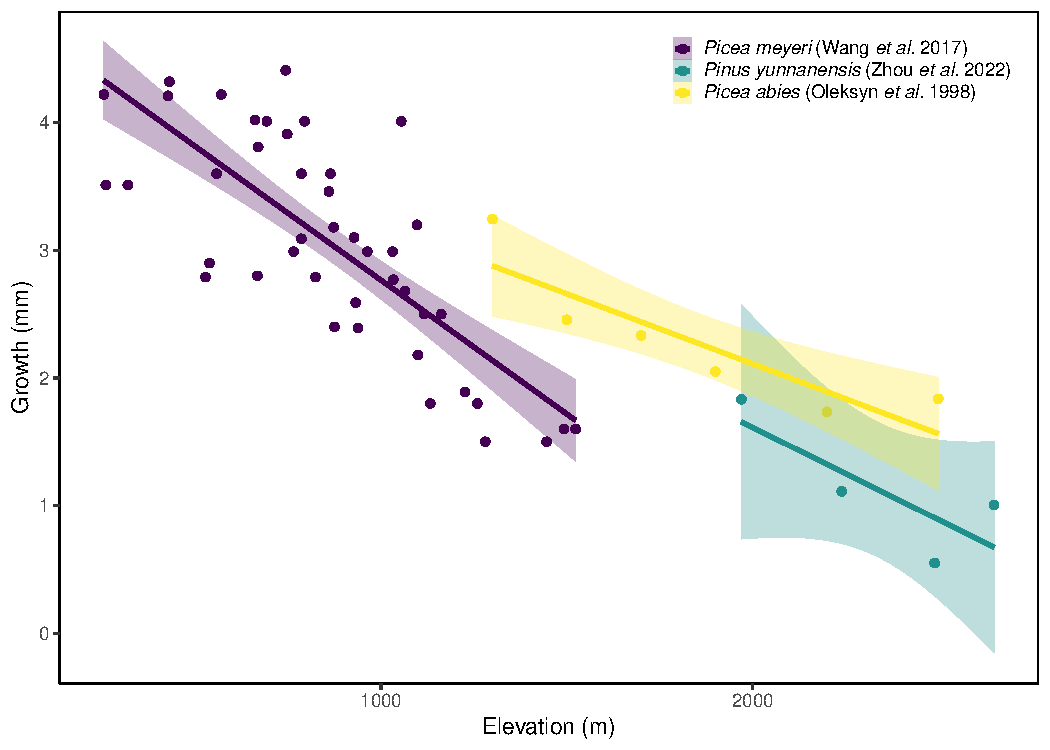
\includegraphics[width=0.7\textwidth]{..//analyses/growthxelevationetc/figures/growthbyelevation_plot.pdf} 
\caption{\emph{Growth $\times$ elevation relationships from the literature.} Simple linear regression fits with 89\% confidence intervals have been added to each dataset. Note that \cite{oleksyn1998growth} measured growth (mm) as diameter at breast height increments, while other studies \citep{wang2017climatic,zhou2022altitudinal} measured growth (mm) as ring width. See `Growth $\times$ elevation relationships' section for more methods details.} 
\end{figure}

\begin{figure}[h!]
% 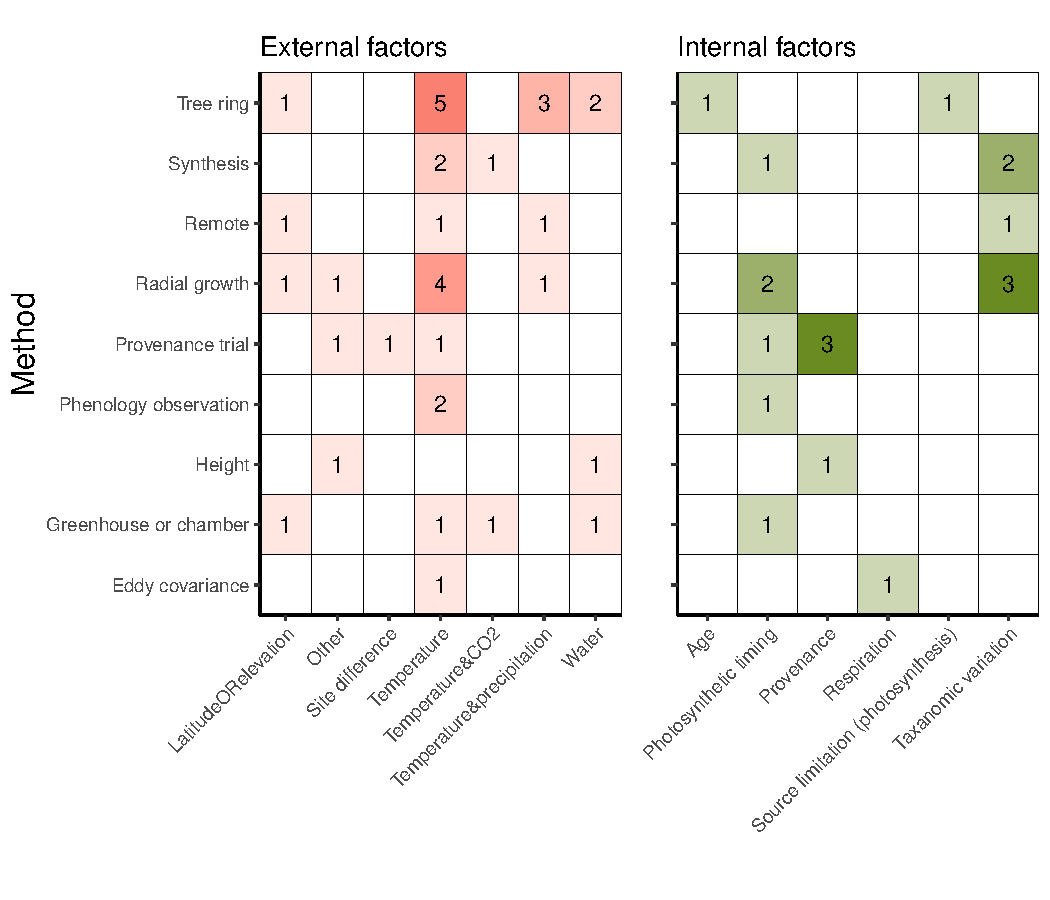
\includegraphics[width=0.8\textwidth]{..//figures/heatmaps/heatmap_combined_endo&exo.pdf}
\caption{\emph{External and internal drivers are frequently but inconsistently studied in the literature.} Review of the prevalence of external (left) and internal (right) drivers mentioned in studies from our literature review, grouped by the general methods used. Many studies tested related hypotheses by measuring different drivers (e.g., latitude or elevation), so we combined similar external and internal factors for clearer comparisons.}
\end{figure}

\begin{figure}[h!]
% 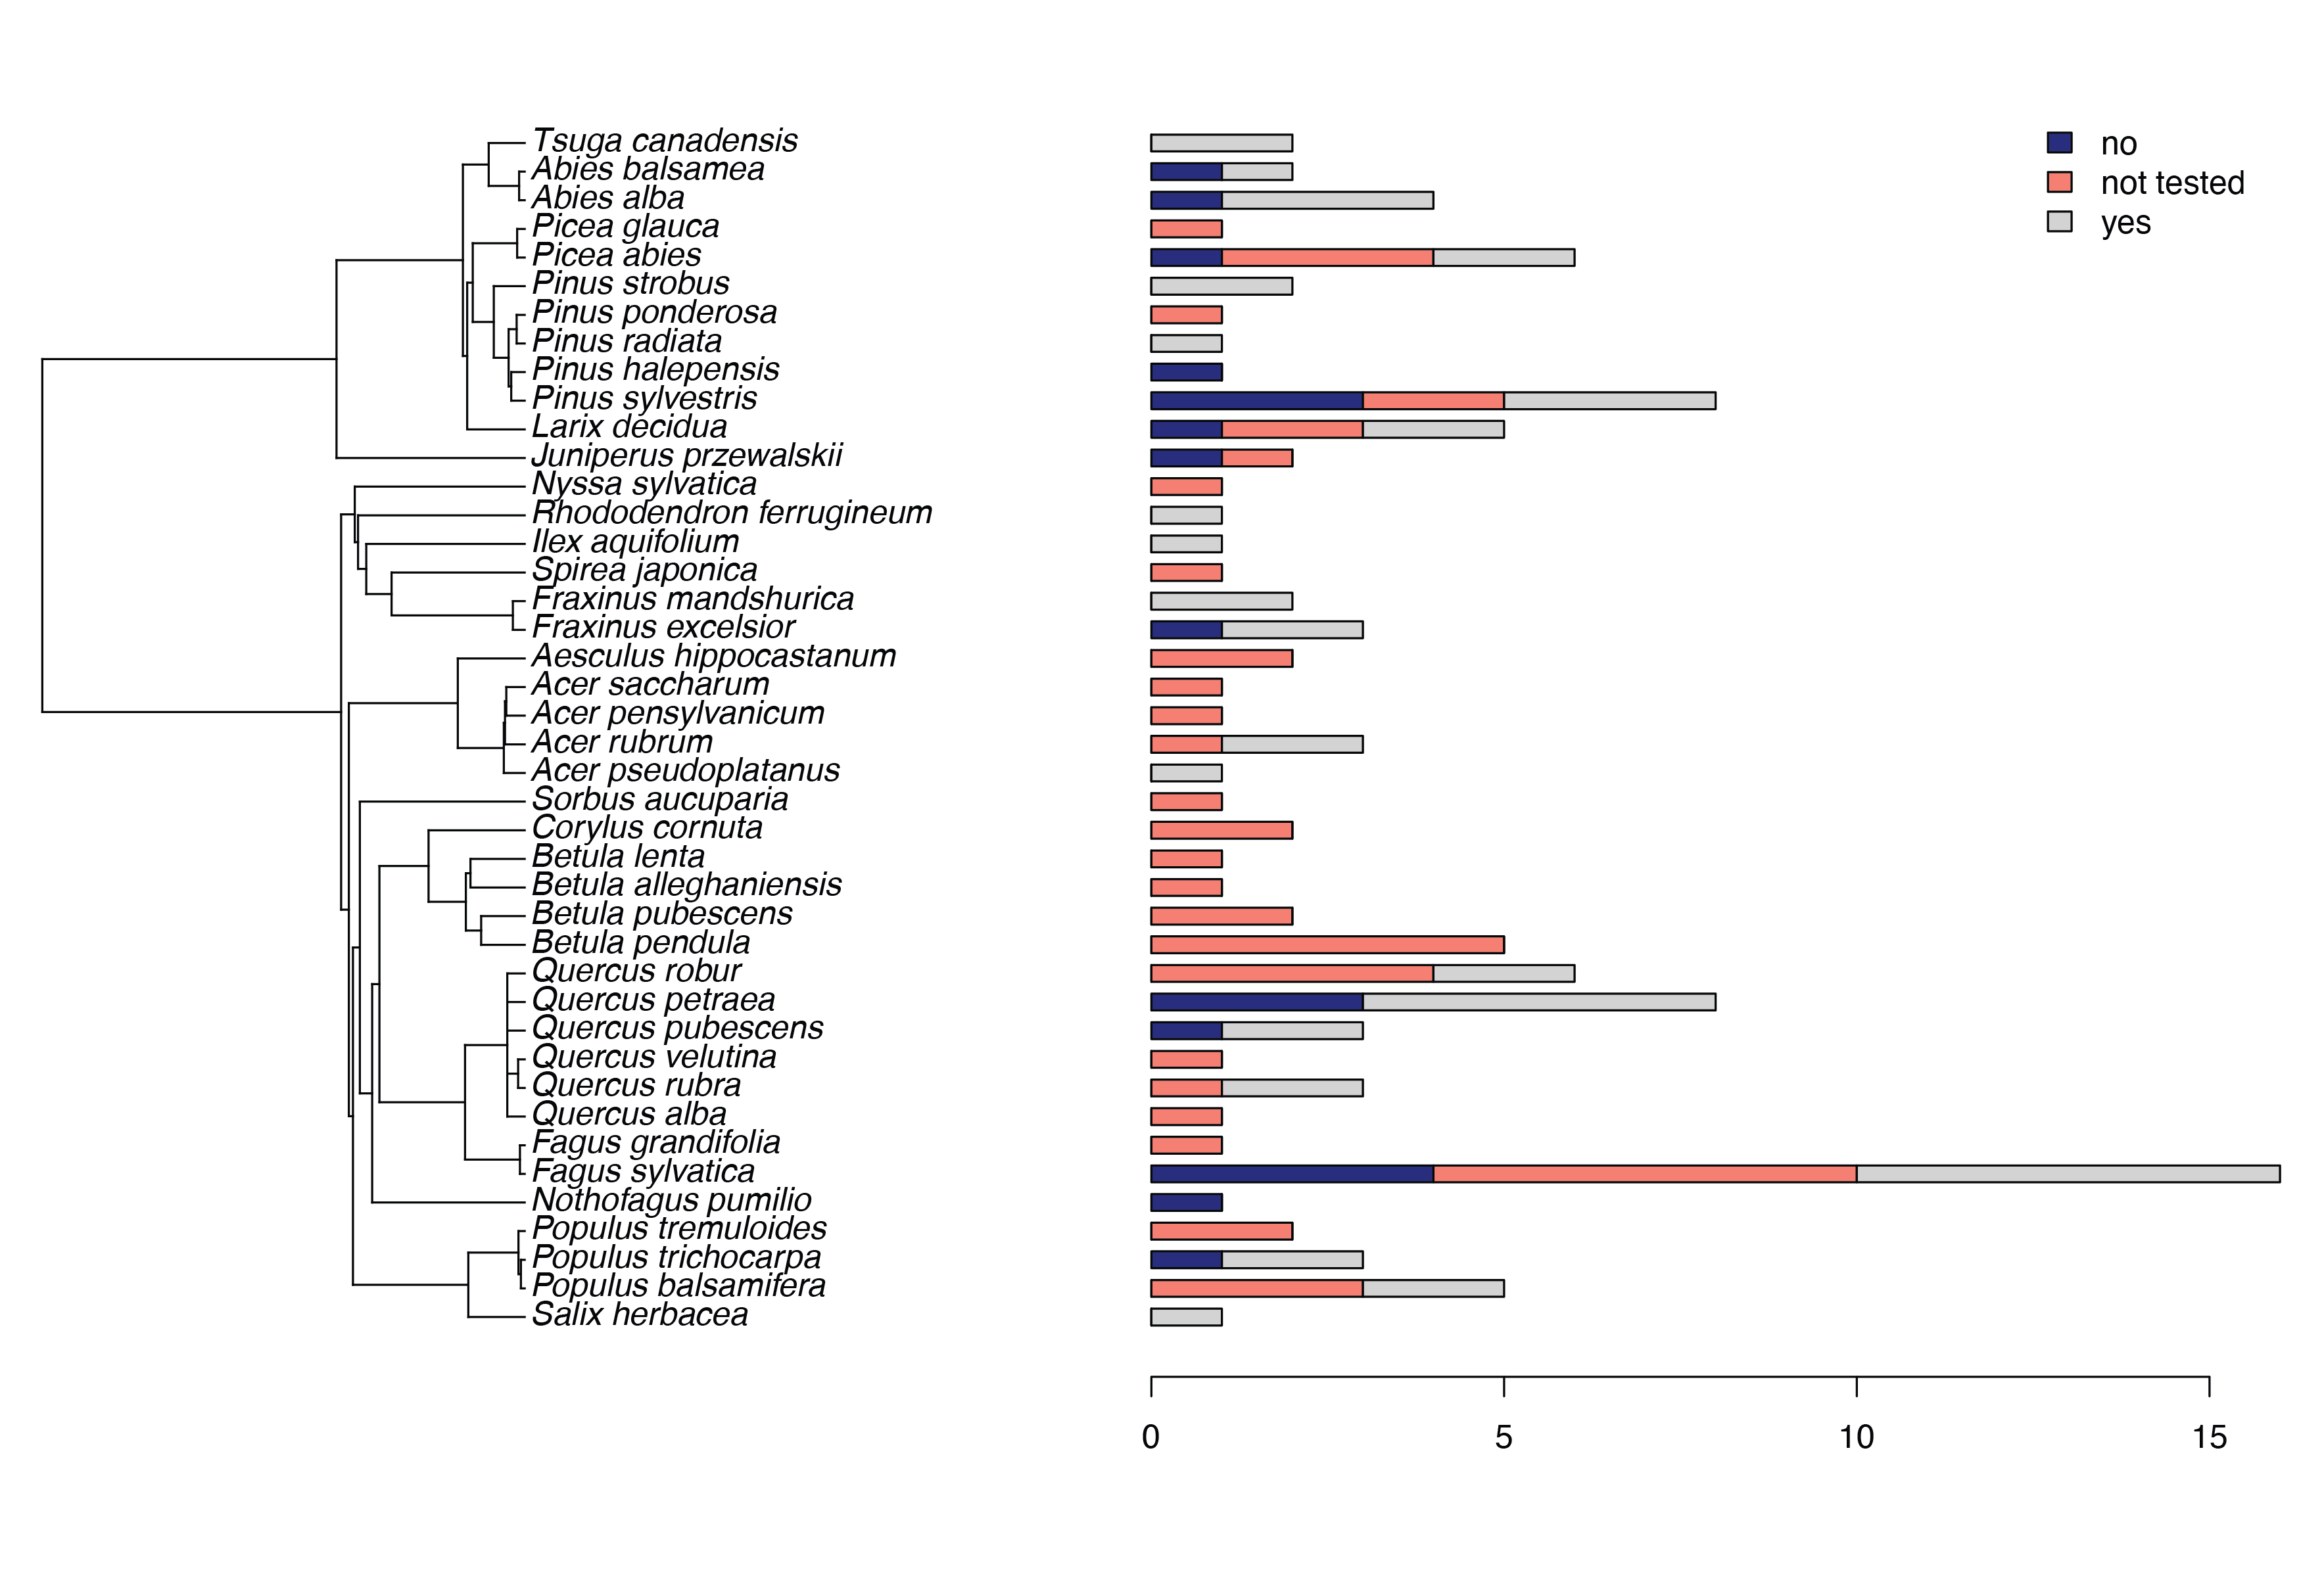
\includegraphics[width=1\textwidth]{..//figures/speciesnumsphylo/phylosppcountsadj.png}  
\caption{\emph{Relationship between growth and growing season length were generally inconsistent across and within species.} Species are shown on the phylogenetic tree from \cite{smith2018constructing}. `Yes' indicates a study found a positive growth $\times$ growing season length relationship, while a `no' means they did not. A number of studies tested relationships possibly related to growth $\times$ growing season length (e.g., spring temperatures relation to growth) but never directly tested growth $\times$ growing season length, which are indicated by `not tested.' We do not show studies which reported species identity only to the genus level.}
\end{figure}

\begin{figure}[h!]
% 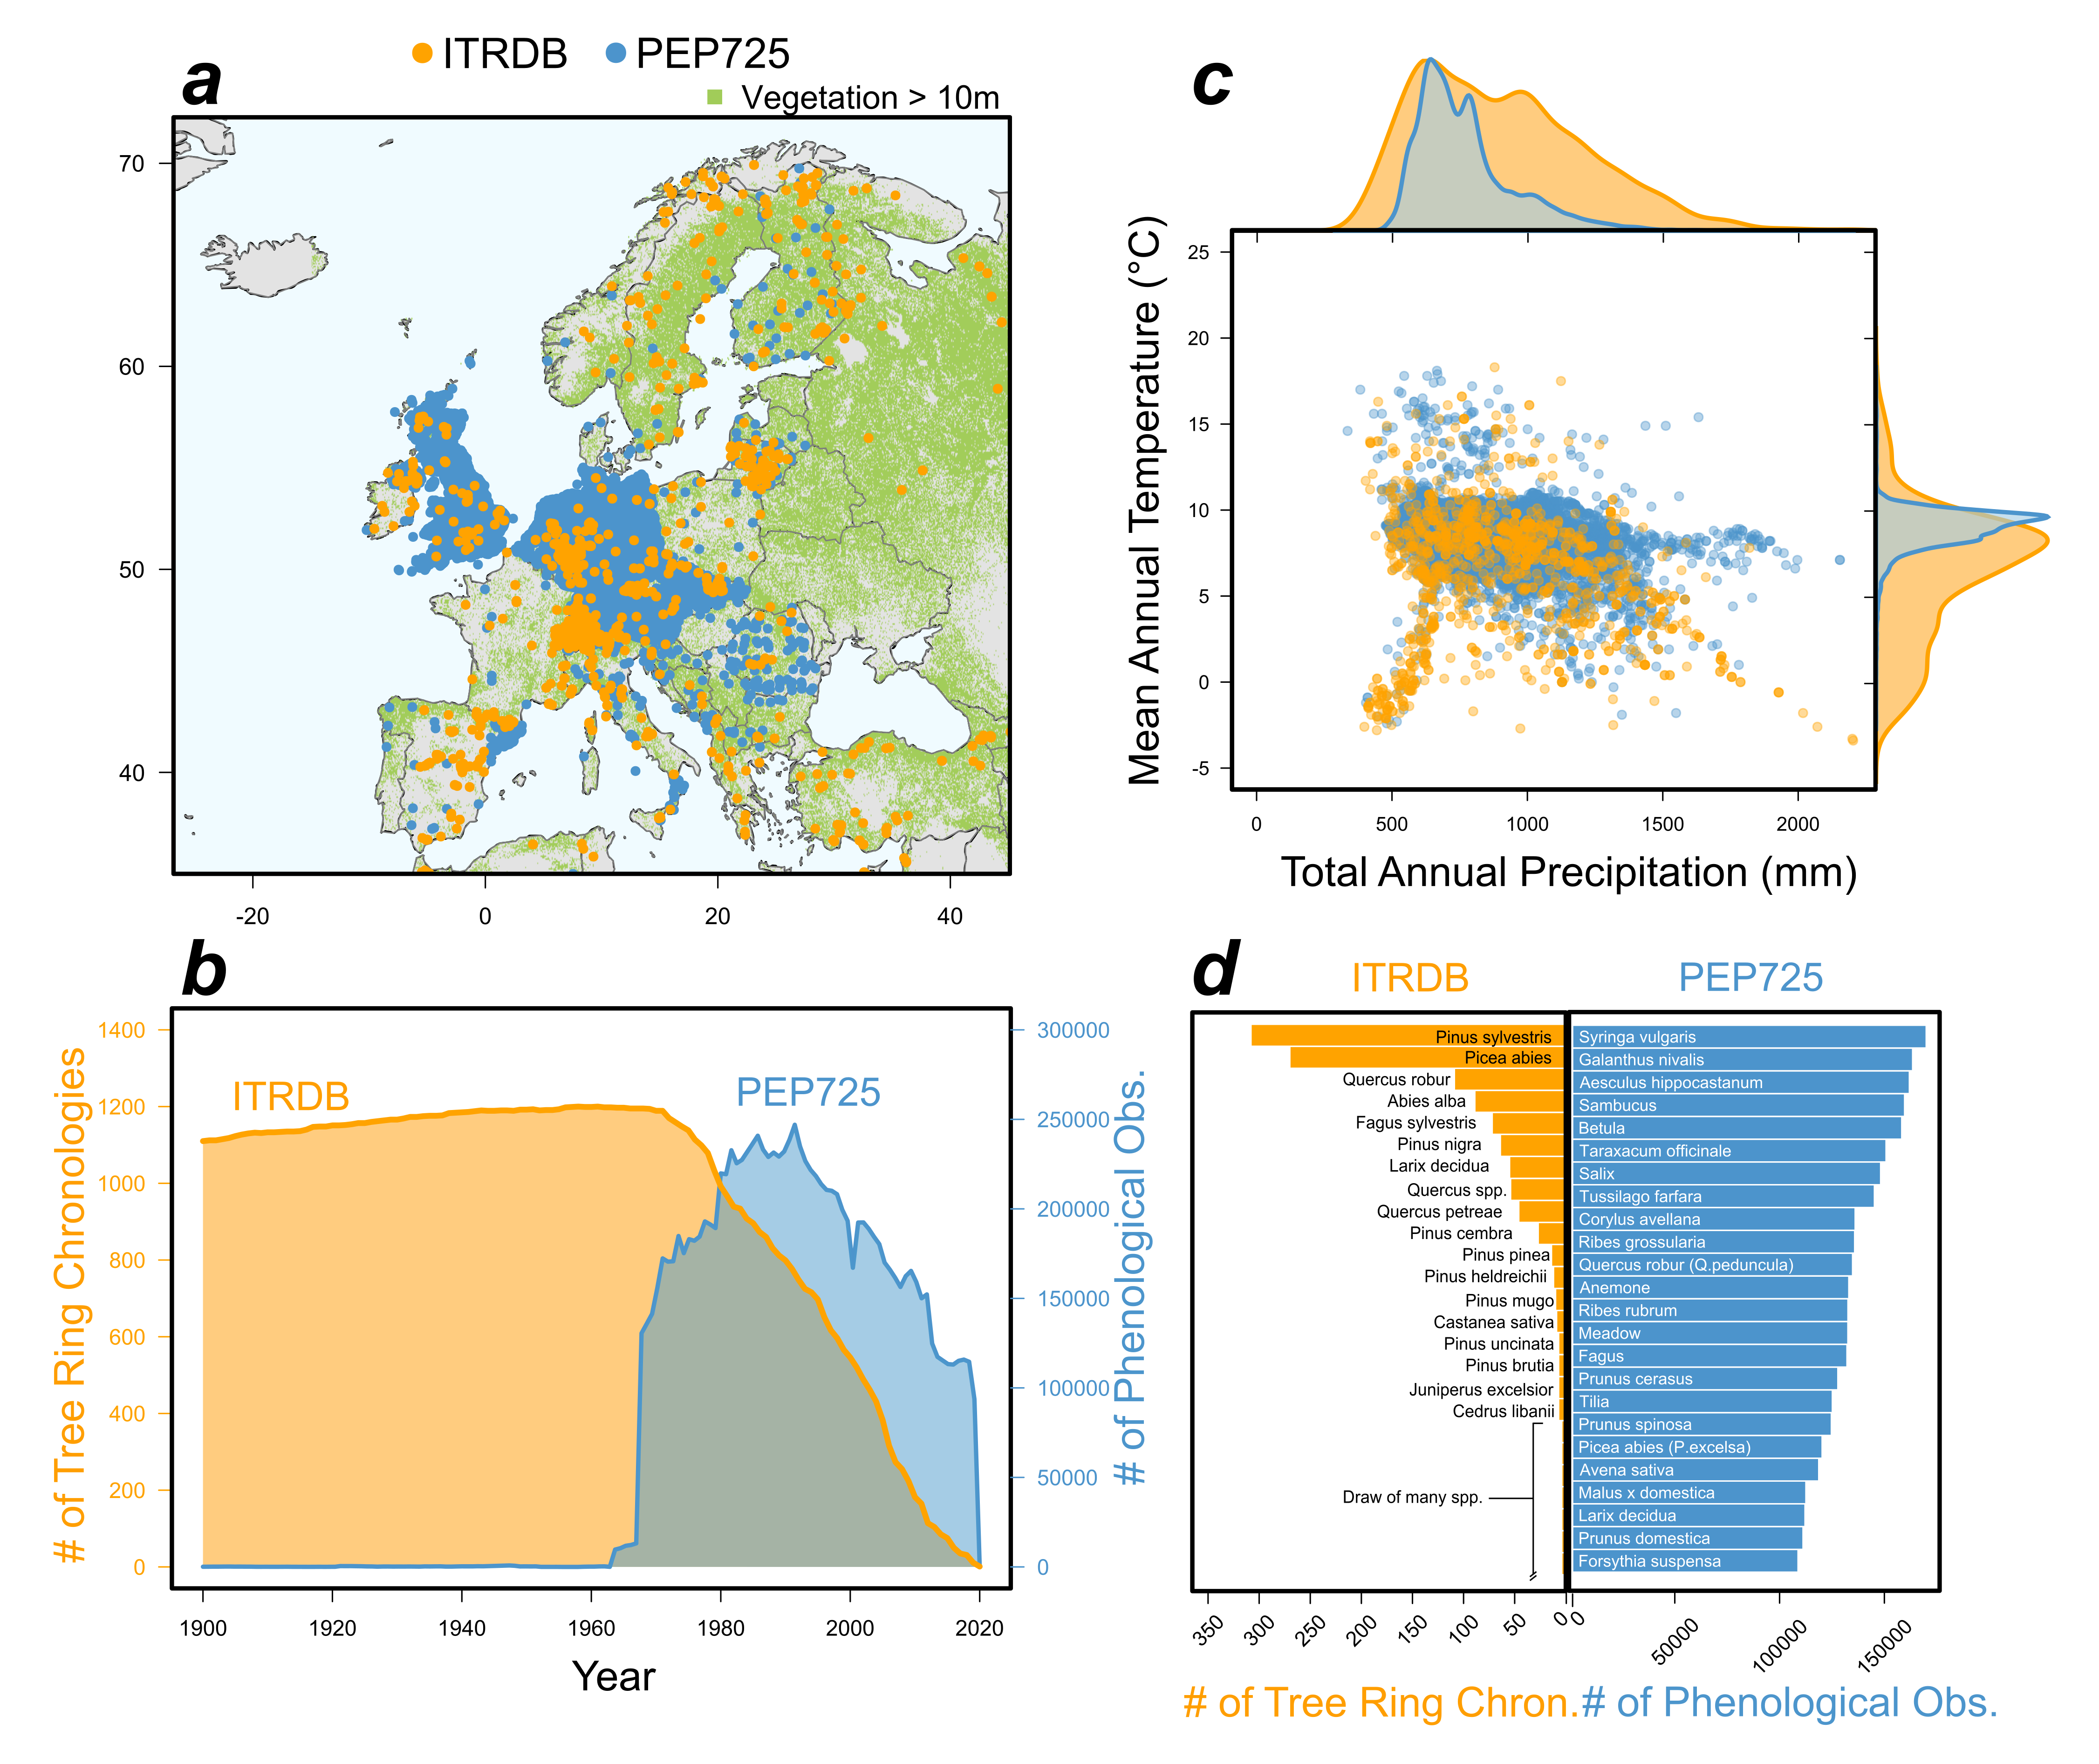
\includegraphics[width=1\textwidth]{..//figures/_figuresFromRuben/itrdb_vs_pep.png} 
\caption{\emph{Data overlap between major growth and phenology databases.} Overlap between two major databases of growth (International Tree Ring Data Bank, ITRDB, orange) and plant phenology (Pan European Phenology Project, PEP725, blue). Both databases are compared in terms of their spatial distributions (a), temporal overlaps (b), coverage of environmental conditions in climate space (c) and taxonomical representation (d). Note that the number of tree ring chronologies in (b) are composed by multiple trees per site, typically 10-20. Climatic data from Worldclim database ver. 2.1 at 2.5\degree grid resolution. PEP725 records in d) show the largest records for any given phenophase per species.}
\end{figure}
\fi

\clearpage
\section*{References}

\begin{thebibliography}{10}
\expandafter\ifx\csname url\endcsname\relax
  \def\url#1{\texttt{#1}}\fi
\expandafter\ifx\csname urlprefix\endcsname\relax\def\urlprefix{URL }\fi
\providecommand{\bibinfo}[2]{#2}
\providecommand{\eprint}[2][]{\url{#2}}

\bibitem{dow2022warm}
\bibinfo{author}{Dow, C.} \emph{et~al.}
\newblock \bibinfo{title}{Warm springs alter timing but not total growth of
  temperate deciduous trees}.
\newblock \emph{\bibinfo{journal}{Nature}} \textbf{\bibinfo{volume}{608}},
  \bibinfo{pages}{552--557} (\bibinfo{year}{2022}).

\bibitem{zohner2023effect}
\bibinfo{author}{Zohner, C.~M.} \emph{et~al.}
\newblock \bibinfo{title}{Effect of climate warming on the timing of autumn
  leaf senescence reverses after the summer solstice}.
\newblock \emph{\bibinfo{journal}{Science}} \textbf{\bibinfo{volume}{381}},
  \bibinfo{pages}{eadf5098} (\bibinfo{year}{2023}).

\bibitem{bruening2017}
\bibinfo{author}{Bruening, J.~B.}, \bibinfo{author}{Tran, T.~J.},
  \bibinfo{author}{Bunn, A.~G.}, \bibinfo{author}{Weiss, S.~B.} \&
  \bibinfo{author}{Salzer, M.~W.}
\newblock \bibinfo{title}{Fine-scale modeling of bristlecone pine treeline
  position in the great basin, usa}.
\newblock \emph{\bibinfo{journal}{Environmental Research Letters}}
  \textbf{\bibinfo{volume}{12}} (\bibinfo{year}{2017}).

\bibitem{oleksyn1998growth}
\bibinfo{author}{Oleksyn, J.} \emph{et~al.}
\newblock \bibinfo{title}{Growth and physiology of picea abies populations from
  elevational transects: common garden evidence for altitudinal ecotypes and
  cold adaptation}.
\newblock \emph{\bibinfo{journal}{Functional Ecology}}
  \textbf{\bibinfo{volume}{12}}, \bibinfo{pages}{573--590}
  (\bibinfo{year}{1998}).

\bibitem{huang2010radial}
\bibinfo{author}{Huang, J.} \emph{et~al.}
\newblock \bibinfo{title}{Radial growth response of four dominant boreal tree
  species to climate along a latitudinal gradient in the eastern canadian
  boreal forest}.
\newblock \emph{\bibinfo{journal}{Global Change Biology}}
  \textbf{\bibinfo{volume}{16}}, \bibinfo{pages}{711--731}
  (\bibinfo{year}{2010}).

\bibitem{cavin2017highest}
\bibinfo{author}{Cavin, L.} \& \bibinfo{author}{Jump, A.~S.}
\newblock \bibinfo{title}{{Highest drought sensitivity and lowest resistance to
  growth suppression are found in the range core of the tree \emph{Fagus
  sylvatica L.} not the equatorial range edge}}.
\newblock \emph{\bibinfo{journal}{Global change biology}}
  \textbf{\bibinfo{volume}{23}}, \bibinfo{pages}{362--379}
  (\bibinfo{year}{2017}).

\bibitem{wang2017climatic}
\bibinfo{author}{Wang, M.} \emph{et~al.}
\newblock \bibinfo{title}{Climatic response of tracheid features of picea
  meyeri along altitude gradient of luyashan mountains of north china}.
\newblock \emph{\bibinfo{journal}{Polish Journal of Ecology}}
  \textbf{\bibinfo{volume}{65}}, \bibinfo{pages}{345--358}
  (\bibinfo{year}{2017}).

\bibitem{zhu2018spatial}
\bibinfo{author}{Zhu, L.} \emph{et~al.}
\newblock \bibinfo{title}{Spatial variability in growth-climate relationships
  of amur cork tree (phellodendron amurense) and their connections with pdo in
  northeast china}.
\newblock \emph{\bibinfo{journal}{Journal of Geophysical Research:
  Biogeosciences}} \textbf{\bibinfo{volume}{123}}, \bibinfo{pages}{1625--1636}
  (\bibinfo{year}{2018}).

\bibitem{zhou2022altitudinal}
\bibinfo{author}{Zhou, Y.} \emph{et~al.}
\newblock \bibinfo{title}{Altitudinal trends in climate change result in radial
  growth variation of pinus yunnanensis at an arid-hot valley of southwest
  china}.
\newblock \emph{\bibinfo{journal}{Dendrochronologia}}
  \textbf{\bibinfo{volume}{71}}, \bibinfo{pages}{125914}
  (\bibinfo{year}{2022}).

\bibitem{smith2014implications}
\bibinfo{author}{Smith, B.} \emph{et~al.}
\newblock \bibinfo{title}{Implications of incorporating n cycling and n
  limitations on primary production in an individual-based dynamic vegetation
  model}.
\newblock \emph{\bibinfo{journal}{Biogeosciences}}
  \textbf{\bibinfo{volume}{11}}, \bibinfo{pages}{2027--2054}
  (\bibinfo{year}{2014}).

\bibitem{chen2000approaches}
\bibinfo{author}{Chen, W.}, \bibinfo{author}{Chen, J.}, \bibinfo{author}{Liu,
  J.} \& \bibinfo{author}{Cihlar, J.}
\newblock \bibinfo{title}{Approaches for reducing uncertainties in regional
  forest carbon balance}.
\newblock \emph{\bibinfo{journal}{Global Biogeochemical Cycles}}
  \textbf{\bibinfo{volume}{14}}, \bibinfo{pages}{827--838}
  (\bibinfo{year}{2000}).

\bibitem{cabon2022cross}
\bibinfo{author}{Cabon, A.} \emph{et~al.}
\newblock \bibinfo{title}{Cross-biome synthesis of source versus sink limits to
  tree growth}.
\newblock \emph{\bibinfo{journal}{Science}} \textbf{\bibinfo{volume}{376}},
  \bibinfo{pages}{758--761} (\bibinfo{year}{2022}).

\bibitem{green2022limits}
\bibinfo{author}{Green, J.~K.} \& \bibinfo{author}{Keenan, T.~F.}
\newblock \bibinfo{title}{The limits of forest carbon sequestration}.
\newblock \emph{\bibinfo{journal}{Science}} \textbf{\bibinfo{volume}{376}},
  \bibinfo{pages}{692--693} (\bibinfo{year}{2022}).

\bibitem{klesse2018sampling}
\bibinfo{author}{Klesse, S.} \emph{et~al.}
\newblock \bibinfo{title}{Sampling bias overestimates climate change impacts on
  forest growth in the southwestern united states}.
\newblock \emph{\bibinfo{journal}{Nature communications}}
  \textbf{\bibinfo{volume}{9}}, \bibinfo{pages}{5336} (\bibinfo{year}{2018}).

\bibitem{nehrbass2014influence}
\bibinfo{author}{Nehrbass-Ahles, C.} \emph{et~al.}
\newblock \bibinfo{title}{The influence of sampling design on tree-ring-based
  quantification of forest growth}.
\newblock \emph{\bibinfo{journal}{Global change biology}}
  \textbf{\bibinfo{volume}{20}}, \bibinfo{pages}{2867--2885}
  (\bibinfo{year}{2014}).

\bibitem{rollinson2021climate}
\bibinfo{author}{Rollinson, C.~R.} \emph{et~al.}
\newblock \bibinfo{title}{Climate sensitivity of understory trees differs from
  overstory trees in temperate mesic forests}.
\newblock \emph{\bibinfo{journal}{Ecology}} \textbf{\bibinfo{volume}{102}},
  \bibinfo{pages}{e03264} (\bibinfo{year}{2021}).

\bibitem{zhao2019international}
\bibinfo{author}{Zhao, S.} \emph{et~al.}
\newblock \bibinfo{title}{The international tree-ring data bank (itrdb)
  revisited: data availability and global ecological representativity}.
\newblock \emph{\bibinfo{journal}{Journal of Biogeography}}
  \textbf{\bibinfo{volume}{46}}, \bibinfo{pages}{355--368}
  (\bibinfo{year}{2019}).

\bibitem{gill2015}
\bibinfo{author}{Gill, A.~L.} \emph{et~al.}
\newblock \bibinfo{title}{Changes in autumn senescence in northern hemisphere
  deciduous trees: a meta-analysis of autumn phenology studies}.
\newblock \emph{\bibinfo{journal}{Annals of Botany}}
  \textbf{\bibinfo{volume}{116}}, \bibinfo{pages}{875--888}
  (\bibinfo{year}{2015}).

\bibitem{locosselli2017dendrobiochemistry}
\bibinfo{author}{Locosselli, G.~M.} \& \bibinfo{author}{Buckeridge, M.~S.}
\newblock \bibinfo{title}{Dendrobiochemistry, a missing link to further
  understand carbon allocation during growth and decline of trees}.
\newblock \emph{\bibinfo{journal}{Trees}} \textbf{\bibinfo{volume}{31}},
  \bibinfo{pages}{1745--1758} (\bibinfo{year}{2017}).

\bibitem{fang2020physiological}
\bibinfo{author}{Fang, J.}, \bibinfo{author}{Lutz, J.~A.},
  \bibinfo{author}{Shugart, H.~H.} \& \bibinfo{author}{Yan, X.}
\newblock \bibinfo{title}{A physiological model for predicting dynamics of tree
  stem-wood non-structural carbohydrates}.
\newblock \emph{\bibinfo{journal}{Journal of Ecology}}
  \textbf{\bibinfo{volume}{108}}, \bibinfo{pages}{702--718}
  (\bibinfo{year}{2020}).

\bibitem{simard2013intra}
\bibinfo{author}{Simard, S.} \emph{et~al.}
\newblock \bibinfo{title}{Intra-annual dynamics of non-structural carbohydrates
  in the cambium of mature conifer trees reflects radial growth demands}.
\newblock \emph{\bibinfo{journal}{Tree Physiology}}
  \textbf{\bibinfo{volume}{33}}, \bibinfo{pages}{913--923}
  (\bibinfo{year}{2013}).

\bibitem{baas2011wood}
\bibinfo{author}{Baas, P.} \& \bibinfo{author}{Wheeler, E.}
\newblock \bibinfo{title}{Wood anatomy and climate change}.
\newblock \emph{\bibinfo{journal}{Climate change, ecology and systematics}}
  \textbf{\bibinfo{volume}{78}}, \bibinfo{pages}{141--155}
  (\bibinfo{year}{2011}).

\bibitem{eckert2019makes}
\bibinfo{author}{Eckert, C.} \emph{et~al.}
\newblock \bibinfo{title}{What makes the wood? exploring the molecular
  mechanisms of xylem acclimation in hardwoods to an ever-changing
  environment}.
\newblock \emph{\bibinfo{journal}{Forests}} \textbf{\bibinfo{volume}{10}},
  \bibinfo{pages}{358} (\bibinfo{year}{2019}).

\bibitem{ensminger2015tree}
\bibinfo{author}{Ensminger, I.}, \bibinfo{author}{Chang, C. Y.-Y.} \&
  \bibinfo{author}{Br{\"a}utigam, K.}
\newblock \bibinfo{title}{Tree responses to environmental cues}.
\newblock \emph{\bibinfo{journal}{Advances in botanical research}}
  \textbf{\bibinfo{volume}{74}}, \bibinfo{pages}{229--263}
  (\bibinfo{year}{2015}).

\bibitem{juvany2013photo}
\bibinfo{author}{Juvany, M.}, \bibinfo{author}{M{\"u}ller, M.} \&
  \bibinfo{author}{Munn{\'e}-Bosch, S.}
\newblock \bibinfo{title}{Photo-oxidative stress in emerging and senescing
  leaves: a mirror image?}
\newblock \emph{\bibinfo{journal}{Journal of experimental botany}}
  \textbf{\bibinfo{volume}{64}}, \bibinfo{pages}{3087--3098}
  (\bibinfo{year}{2013}).

\bibitem{camarero2022decoupled}
\bibinfo{author}{Camarero, J.~J.} \emph{et~al.}
\newblock \bibinfo{title}{Decoupled leaf-wood phenology in two pine species
  from contrasting climates: Longer growing seasons do not mean more radial
  growth}.
\newblock \emph{\bibinfo{journal}{Agricultural and Forest Meteorology}}
  \textbf{\bibinfo{volume}{327}}, \bibinfo{pages}{109223}
  (\bibinfo{year}{2022}).

\bibitem{chen2000}
\bibinfo{author}{Chen, J.}, \bibinfo{author}{Chen, W.}, \bibinfo{author}{Liu,
  J.}, \bibinfo{author}{Cihlar, J.} \& \bibinfo{author}{Gray, S.}
\newblock \bibinfo{title}{Annual carbon balance of canada's forests during
  1895-1996}.
\newblock \emph{\bibinfo{journal}{Global Biogeochemical Cycles}}
  \textbf{\bibinfo{volume}{14}}, \bibinfo{pages}{839--849}
  (\bibinfo{year}{2000}).

\bibitem{vcufar2015variations}
\bibinfo{author}{{\v{C}}ufar, K.} \emph{et~al.}
\newblock \bibinfo{title}{{Do variations in leaf phenology affect radial growth
  variations in \emph{Fagus sylvatica}?}}
\newblock \emph{\bibinfo{journal}{International journal of biometeorology}}
  \textbf{\bibinfo{volume}{59}}, \bibinfo{pages}{1127--1132}
  (\bibinfo{year}{2015}).

\bibitem{delpierre2017tree}
\bibinfo{author}{Delpierre, N.}, \bibinfo{author}{Guillemot, J.},
  \bibinfo{author}{Dufr{\^e}ne, E.}, \bibinfo{author}{Cecchini, S.} \&
  \bibinfo{author}{Nicolas, M.}
\newblock \bibinfo{title}{Tree phenological ranks repeat from year to year and
  correlate with growth in temperate deciduous forests}.
\newblock \emph{\bibinfo{journal}{Agricultural and Forest Meteorology}}
  \textbf{\bibinfo{volume}{234}}, \bibinfo{pages}{1--10}
  (\bibinfo{year}{2017}).

\bibitem{de2022temperature}
\bibinfo{author}{de~Sauvage, J.~C.}, \bibinfo{author}{Vitasse, Y.},
  \bibinfo{author}{Meier, M.}, \bibinfo{author}{Delzon, S.} \&
  \bibinfo{author}{Bigler, C.}
\newblock \bibinfo{title}{Temperature rather than individual growing period
  length determines radial growth of sessile oak in the pyrenees}.
\newblock \emph{\bibinfo{journal}{Agricultural and Forest Meteorology}}
  \textbf{\bibinfo{volume}{317}}, \bibinfo{pages}{108885}
  (\bibinfo{year}{2022}).

\bibitem{gao2022earlier}
\bibinfo{author}{Gao, S.} \emph{et~al.}
\newblock \bibinfo{title}{An earlier start of the thermal growing season
  enhances tree growth in cold humid areas but not in dry areas}.
\newblock \emph{\bibinfo{journal}{Nature ecology \& evolution}}
  \textbf{\bibinfo{volume}{6}}, \bibinfo{pages}{397--404}
  (\bibinfo{year}{2022}).

\bibitem{grossiord2022warming}
\bibinfo{author}{Grossiord, C.} \emph{et~al.}
\newblock \bibinfo{title}{Warming may extend tree growing seasons and
  compensate for reduced carbon uptake during dry periods}.
\newblock \emph{\bibinfo{journal}{Journal of Ecology}}
  \textbf{\bibinfo{volume}{110}}, \bibinfo{pages}{1575--1589}
  (\bibinfo{year}{2022}).

\bibitem{keenan2014net}
\bibinfo{author}{Keenan, T.~F.} \emph{et~al.}
\newblock \bibinfo{title}{Net carbon uptake has increased through
  warming-induced changes in temperate forest phenology}.
\newblock \emph{\bibinfo{journal}{Nature Climate Change}}
  \textbf{\bibinfo{volume}{4}}, \bibinfo{pages}{598--604}
  (\bibinfo{year}{2014}).

\bibitem{silvestro2023longer}
\bibinfo{author}{Silvestro, R.} \emph{et~al.}
\newblock \bibinfo{title}{A longer wood growing season does not lead to higher
  carbon sequestration}.
\newblock \emph{\bibinfo{journal}{Scientific reports}}
  \textbf{\bibinfo{volume}{13}}, \bibinfo{pages}{4059} (\bibinfo{year}{2023}).

\bibitem{wheeler2016snow}
\bibinfo{author}{Wheeler, J.~A.} \emph{et~al.}
\newblock \bibinfo{title}{The snow and the willows: earlier spring snowmelt
  reduces performance in the low-lying alpine shrub salix herbacea}.
\newblock \emph{\bibinfo{journal}{Journal of Ecology}}
  \textbf{\bibinfo{volume}{104}}, \bibinfo{pages}{1041--1050}
  (\bibinfo{year}{2016}).

\bibitem{brand2022}
\bibinfo{author}{Brand, R.}, \bibinfo{author}{Srur, A.~M.} \&
  \bibinfo{author}{Villalba, R.}
\newblock \bibinfo{title}{{Contrasting growth trends in \emph{Nothofagus
  pumilio} upper-elevation forests induced by climate warming in the Southern
  Andes}}.
\newblock \emph{\bibinfo{journal}{Agricultural and Forest Meteorology}}
  \textbf{\bibinfo{volume}{323}} (\bibinfo{year}{2022}).

\bibitem{buermann2018widespread}
\bibinfo{author}{Buermann, W.} \emph{et~al.}
\newblock \bibinfo{title}{Widespread seasonal compensation effects of spring
  warming on northern plant productivity}.
\newblock \emph{\bibinfo{journal}{Nature}} \textbf{\bibinfo{volume}{562}},
  \bibinfo{pages}{110--114} (\bibinfo{year}{2018}).

\bibitem{drew2018growth}
\bibinfo{author}{Drew, D.} \& \bibinfo{author}{Downes, G.}
\newblock \bibinfo{title}{Growth at the microscale: long term thinning effects
  on patterns and timing of intra-annual stem increment in radiata pine. for
  ecosyst 5: 32} (\bibinfo{year}{2018}).

\bibitem{eckes2021}
\bibinfo{author}{Eckes-Shephard, A.~H.}, \bibinfo{author}{Tiavlovsky, E.},
  \bibinfo{author}{Chen, Y.}, \bibinfo{author}{Fonti, P.} \&
  \bibinfo{author}{Friend, A.~D.}
\newblock \bibinfo{title}{Direct response of tree growth to soil water and its
  implications for terrestrial carbon cycle modelling}.
\newblock \emph{\bibinfo{journal}{Global Change Biology}}
  \textbf{\bibinfo{volume}{27}}, \bibinfo{pages}{121--135}
  (\bibinfo{year}{2021}).

\bibitem{etzold2022number}
\bibinfo{author}{Etzold, S.} \emph{et~al.}
\newblock \bibinfo{title}{Number of growth days and not length of the growth
  period determines radial stem growth of temperate trees}.
\newblock \emph{\bibinfo{journal}{Ecology Letters}}
  \textbf{\bibinfo{volume}{25}}, \bibinfo{pages}{427--439}
  (\bibinfo{year}{2022}).

\bibitem{kolavr2016response}
\bibinfo{author}{Kol{\'a}{\v{r}}, T.} \emph{et~al.}
\newblock \bibinfo{title}{Response of the leaf phenology and tree-ring width of
  european beech to climate variability}.
\newblock \emph{\bibinfo{journal}{Silva Fennica}} \textbf{\bibinfo{volume}{50}}
  (\bibinfo{year}{2016}).

\bibitem{oddi2022contrasting}
\bibinfo{author}{Oddi, L.} \emph{et~al.}
\newblock \bibinfo{title}{Contrasting responses of forest growth and carbon
  sequestration to heat and drought in the alps}.
\newblock \emph{\bibinfo{journal}{Environmental Research Letters}}
  \textbf{\bibinfo{volume}{17}}, \bibinfo{pages}{045015}
  (\bibinfo{year}{2022}).

\bibitem{zhu2021different}
\bibinfo{author}{Zhu, L.} \emph{et~al.}
\newblock \bibinfo{title}{Different response of earlywood vessel features of
  fraxinus mandshurica to rapid warming in warm-dry and cold-wet areas}.
\newblock \emph{\bibinfo{journal}{Agricultural and Forest Meteorology}}
  \textbf{\bibinfo{volume}{307}}, \bibinfo{pages}{108523}
  (\bibinfo{year}{2021}).

\bibitem{finzi2020}
\bibinfo{author}{Finzi, A.~C.} \emph{et~al.}
\newblock \bibinfo{title}{Carbon budget of the harvard forest long-term
  ecological research site: pattern, process, and response to global change}.
\newblock \emph{\bibinfo{journal}{Ecological Monographs}}
  \textbf{\bibinfo{volume}{90}} (\bibinfo{year}{2020}).

\bibitem{moser2010timing}
\bibinfo{author}{Moser, L.} \emph{et~al.}
\newblock \bibinfo{title}{Timing and duration of european larch growing season
  along altitudinal gradients in the swiss alps}.
\newblock \emph{\bibinfo{journal}{Tree physiology}}
  \textbf{\bibinfo{volume}{30}}, \bibinfo{pages}{225--233}
  (\bibinfo{year}{2010}).

\bibitem{richardson2010influence}
\bibinfo{author}{Richardson, A.~D.} \emph{et~al.}
\newblock \bibinfo{title}{Influence of spring and autumn phenological
  transitions on forest ecosystem productivity}.
\newblock \emph{\bibinfo{journal}{Philosophical Transactions of the Royal
  Society B: Biological Sciences}} \textbf{\bibinfo{volume}{365}},
  \bibinfo{pages}{3227--3246} (\bibinfo{year}{2010}).

\bibitem{soolanayakanahally2013timing}
\bibinfo{author}{Soolanayakanahally, R.~Y.}, \bibinfo{author}{Guy, R.~D.},
  \bibinfo{author}{Silim, S.~N.} \& \bibinfo{author}{Song, M.}
\newblock \bibinfo{title}{Timing of photoperiodic competency causes
  phenological mismatch in balsam poplar (populus balsamifera l.)}.
\newblock \emph{\bibinfo{journal}{Plant, cell \& environment}}
  \textbf{\bibinfo{volume}{36}}, \bibinfo{pages}{116--127}
  (\bibinfo{year}{2013}).

\bibitem{stridbeck2022}
\bibinfo{author}{Stridbeck, P.} \emph{et~al.}
\newblock \bibinfo{title}{{Partly decoupled tree-ring width and leaf phenology
  response to 20th century temperature change in Sweden}}.
\newblock \emph{\bibinfo{journal}{Dendrochronologia}}
  \textbf{\bibinfo{volume}{75}} (\bibinfo{year}{2022}).

\bibitem{zhang2021drought}
\bibinfo{author}{Zhang, J.} \emph{et~al.}
\newblock \bibinfo{title}{Drought limits wood production of juniperus
  przewalskii even as growing seasons lengthens in a cold and arid
  environment}.
\newblock \emph{\bibinfo{journal}{Catena}} \textbf{\bibinfo{volume}{196}},
  \bibinfo{pages}{104936} (\bibinfo{year}{2021}).

\bibitem{zani2020increased}
\bibinfo{author}{Zani, D.}, \bibinfo{author}{Crowther, T.~W.},
  \bibinfo{author}{Mo, L.}, \bibinfo{author}{Renner, S.~S.} \&
  \bibinfo{author}{Zohner, C.~M.}
\newblock \bibinfo{title}{Increased growing-season productivity drives earlier
  autumn leaf senescence in temperate trees}.
\newblock \emph{\bibinfo{journal}{Science}} \textbf{\bibinfo{volume}{370}},
  \bibinfo{pages}{1066--1071} (\bibinfo{year}{2020}).

\bibitem{zohner2020interactive}
\bibinfo{author}{Zohner, C.~M.}, \bibinfo{author}{Mo, L.},
  \bibinfo{author}{Pugh, T.~A.}, \bibinfo{author}{Bastin, J.-F.} \&
  \bibinfo{author}{Crowther, T.~W.}
\newblock \bibinfo{title}{Interactive climate factors restrict future increases
  in spring productivity of temperate and boreal trees}.
\newblock \emph{\bibinfo{journal}{Global change biology}}
  \textbf{\bibinfo{volume}{26}}, \bibinfo{pages}{4042--4055}
  (\bibinfo{year}{2020}).

\bibitem{cuny2012life}
\bibinfo{author}{Cuny, H.~E.}, \bibinfo{author}{Rathgeber, C.~B.},
  \bibinfo{author}{Lebourgeois, F.}, \bibinfo{author}{Fortin, M.} \&
  \bibinfo{author}{Fournier, M.}
\newblock \bibinfo{title}{Life strategies in intra-annual dynamics of wood
  formation: example of three conifer species in a temperate forest in
  north-east france}.
\newblock \emph{\bibinfo{journal}{Tree physiology}}
  \textbf{\bibinfo{volume}{32}}, \bibinfo{pages}{612--625}
  (\bibinfo{year}{2012}).

\bibitem{francon2020}
\bibinfo{author}{Francon, L.} \emph{et~al.}
\newblock \bibinfo{title}{Assessing the effects of earlier snow melt-out on
  alpine shrub growth: The sooner the better?}
\newblock \emph{\bibinfo{journal}{Ecological Indicators}}
  \textbf{\bibinfo{volume}{115}} (\bibinfo{year}{2020}).

\bibitem{michelot2012comparing}
\bibinfo{author}{Michelot, A.}, \bibinfo{author}{Simard, S.},
  \bibinfo{author}{Rathgeber, C.}, \bibinfo{author}{Dufr{\^e}ne, E.} \&
  \bibinfo{author}{Damesin, C.}
\newblock \bibinfo{title}{{Comparing the intra-annual wood formation of three
  European species (\emph{Fagus sylvatica, Quercus petraea and Pinus
  sylvestris}) as related to leaf phenology and non-structural carbohydrate
  dynamics}}.
\newblock \emph{\bibinfo{journal}{Tree physiology}}
  \textbf{\bibinfo{volume}{32}}, \bibinfo{pages}{1033--1045}
  (\bibinfo{year}{2012}).

\bibitem{ren2019}
\bibinfo{author}{Ren, P.} \emph{et~al.}
\newblock \bibinfo{title}{Growth rate rather than growing season length
  determines wood biomass in dry environments}.
\newblock \emph{\bibinfo{journal}{Agricultural and Forest Meteorology}}
  \textbf{\bibinfo{volume}{271}}, \bibinfo{pages}{46--53}
  (\bibinfo{year}{2019}).

\bibitem{sebazc2020}
\bibinfo{author}{Sebastian-Azcona, J.}, \bibinfo{author}{Hacke, U.} \&
  \bibinfo{author}{Hamann, A.}
\newblock \bibinfo{title}{Xylem anomalies as indicators of maladaptation to
  climate in forest trees: Implications for assisted migration}.
\newblock \emph{\bibinfo{journal}{Frontiers in Plant Science}}
  \textbf{\bibinfo{volume}{11}} (\bibinfo{year}{2020}).

\bibitem{vitasse2009altitudinal}
\bibinfo{author}{Vitasse, Y.}, \bibinfo{author}{Delzon, S.},
  \bibinfo{author}{Bresson, C.~C.}, \bibinfo{author}{Michalet, R.} \&
  \bibinfo{author}{Kremer, A.}
\newblock \bibinfo{title}{Altitudinal differentiation in growth and phenology
  among populations of temperate-zone tree species growing in a common garden}.
\newblock \emph{\bibinfo{journal}{Canadian Journal of Forest Research}}
  \textbf{\bibinfo{volume}{39}}, \bibinfo{pages}{1259--1269}
  (\bibinfo{year}{2009}).

\bibitem{chen1999effects}
\bibinfo{author}{Chen, W.} \emph{et~al.}
\newblock \bibinfo{title}{Effects of climatic variability on the annual carbon
  sequestration by a boreal aspen forest}.
\newblock \emph{\bibinfo{journal}{Global Change Biology}}
  \textbf{\bibinfo{volume}{5}}, \bibinfo{pages}{41--53} (\bibinfo{year}{1999}).

\bibitem{mckown2016impacts}
\bibinfo{author}{McKown, A.~D.}, \bibinfo{author}{Guy, R.~D.} \&
  \bibinfo{author}{Quamme, L.~K.}
\newblock \bibinfo{title}{Impacts of bud set and lammas phenology on root:
  shoot biomass partitioning and carbon gain physiology in poplar}.
\newblock \emph{\bibinfo{journal}{Trees}} \textbf{\bibinfo{volume}{30}},
  \bibinfo{pages}{2131--2141} (\bibinfo{year}{2016}).

\bibitem{smith2018constructing}
\bibinfo{author}{Smith, S.~A.} \& \bibinfo{author}{Brown, J.~W.}
\newblock \bibinfo{title}{Constructing a broadly inclusive seed plant
  phylogeny}.
\newblock \emph{\bibinfo{journal}{American journal of botany}}
  \textbf{\bibinfo{volume}{105}}, \bibinfo{pages}{302--314}
  (\bibinfo{year}{2018}).

\end{thebibliography}

\bibliographystyle{naturemag}

\end{document}


